\begin{figure}[H]
\centering
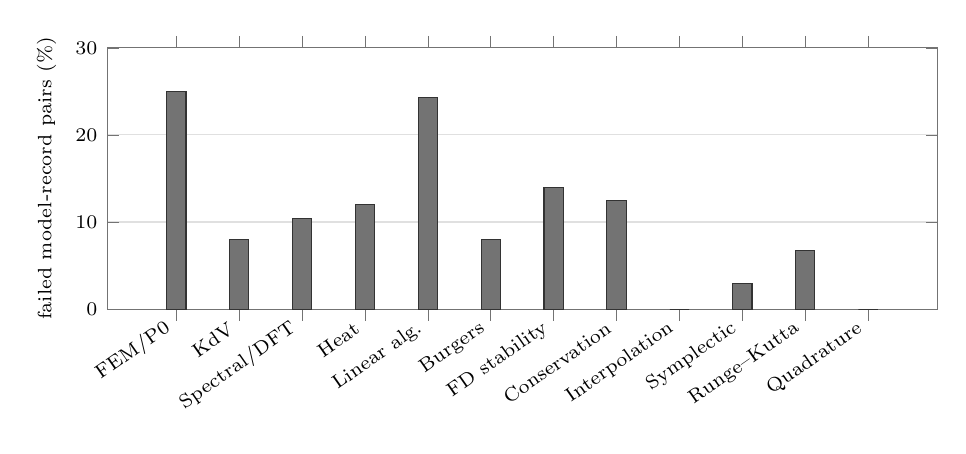
\begin{tikzpicture}
\begin{axis}[
  ybar,
  width=\linewidth,
  height=4.9cm,
  bar width=7pt,
  ymin=0,
  ymax=30,
  ylabel={failed model-record pairs (\%)},
  symbolic x coords={{FEM/P0},{KdV},{Spectral/DFT},{Heat},{Linear alg.},{Burgers},{FD stability},{Conservation},{Interpolation},{Symplectic},{Runge--Kutta},{Quadrature}},
  xtick=data,
  x tick label style={rotate=35, anchor=east, font=\scriptsize},
  tick label style={font=\scriptsize},
  label style={font=\scriptsize},
  ymajorgrids=true,
  grid style={black!12},
  axis line style={black!55},
  tick style={black!55}
]
\addplot+[draw=black!80, fill=black!55] coordinates {
({FEM/P0},25.0)
({KdV},8.0)
({Spectral/DFT},10.4)
({Heat},12.0)
({Linear alg.},24.3)
({Burgers},8.0)
({FD stability},14.0)
({Conservation},12.5)
({Interpolation},0)
({Symplectic},2.9)
({Runge--Kutta},6.7)
({Quadrature},0)
};
\end{axis}
\end{tikzpicture}
\caption{Failure rate by theorem family in the May-2026 5-model proof panel.
Failures concentrate in FEM/P0 projection, linear-algebra stability, FD
stability, conservation, heat/CFL, and spectral/DFT rows rather than uniformly
across families.}
\label{fig:coverage-failure}
\end{figure}
